\graphicspath{
  {./images/bmps/}{./images/vects/}{./images/}
  {./images/presentation/bmps/}{./images/presentation/vects/}{./images/presentation/}
  {./images/chapter00/bmps/}{./images/chapter00/vects/}{./images/chapter00/}
  {./images/chapter07/bmps/}{./images/chapter07/vects/}{./images/chapter07/}
}

\subsection{Local Planning}

\begin{frame}{Pipeline}
   \begin{center}
    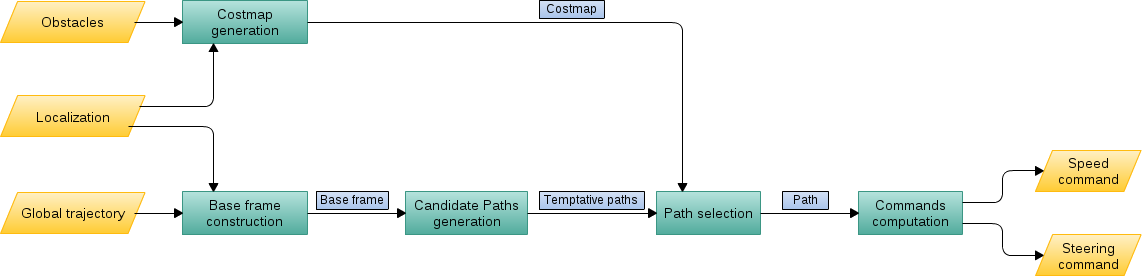
\includegraphics[width=\textwidth]{pipeline_cp07}
  \end{center}
  
  \note {

  }
\end{frame}

\begin{frame}{Costmap generation}
   \begin{center}
    \begin{equation}\nonumber
      \mathcal{C}(i, j) = \exp (-1.0 \cdot \alpha \cdot ( \|c_{ij}-\vec{o}\| - \rho_{inscribed})) \cdot 253
    \end{equation}\\~\\
    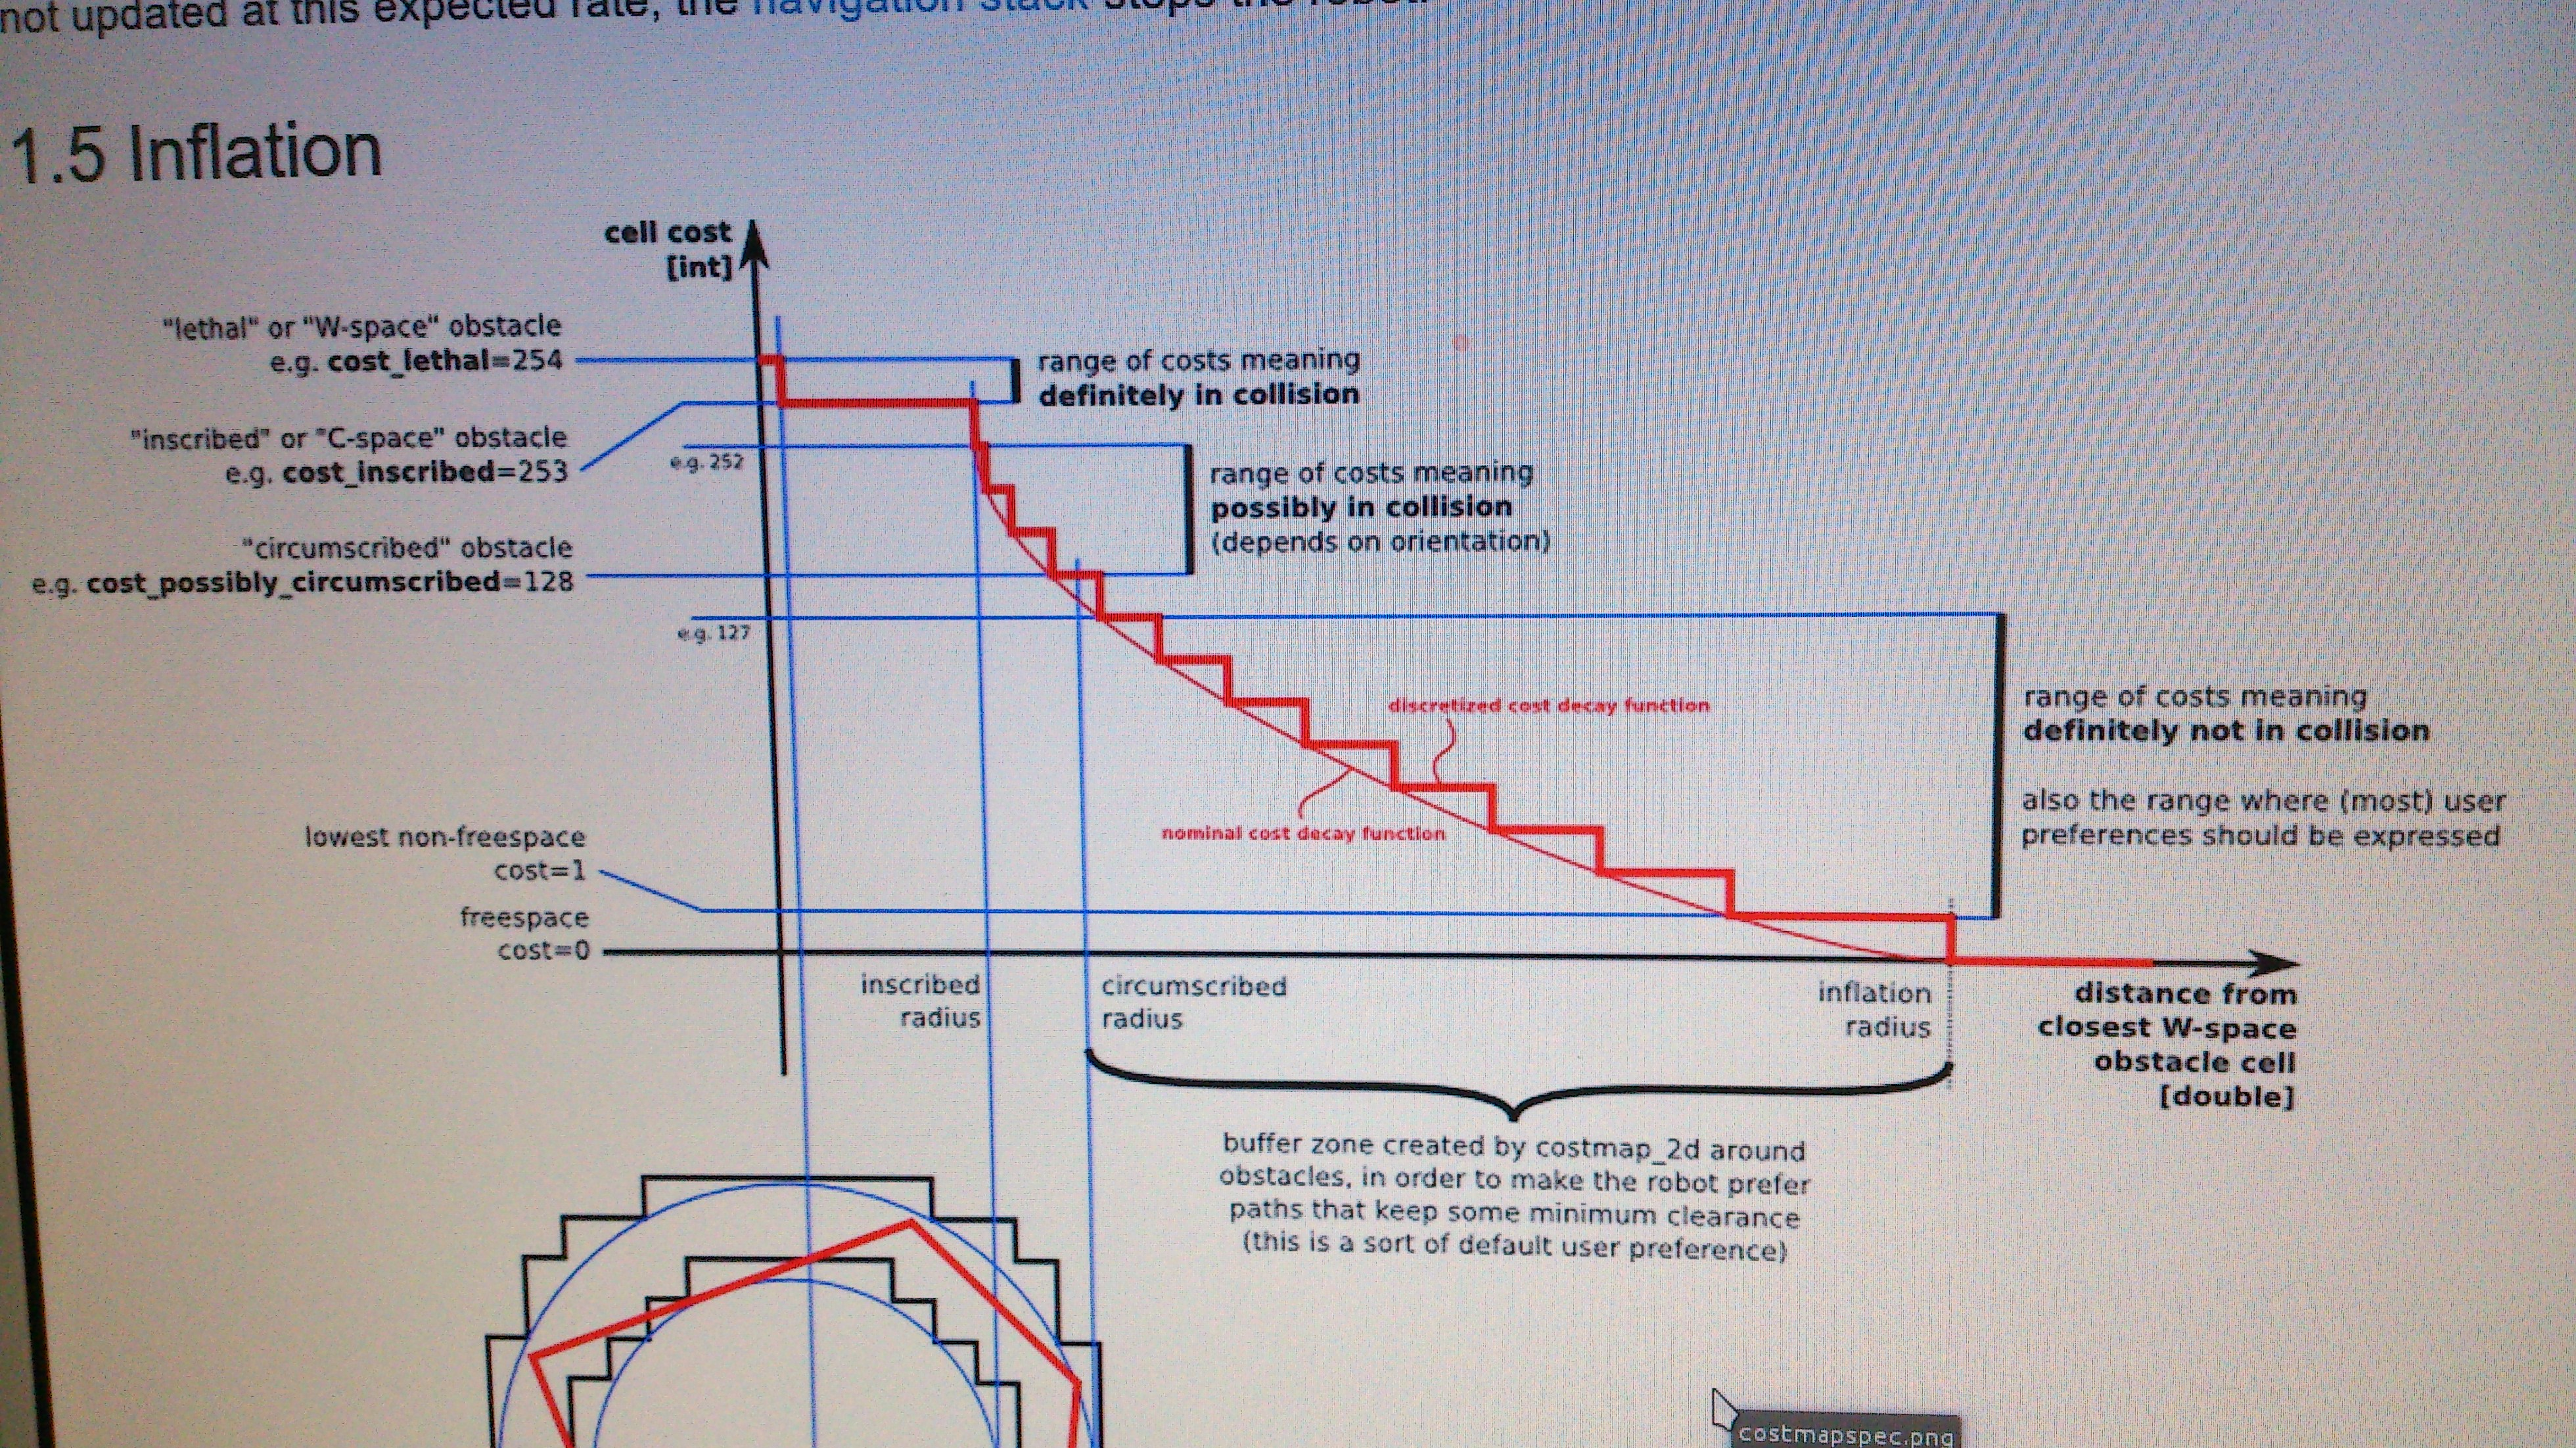
\includegraphics[height=0.5\textheight]{cost_levels}
    ~
    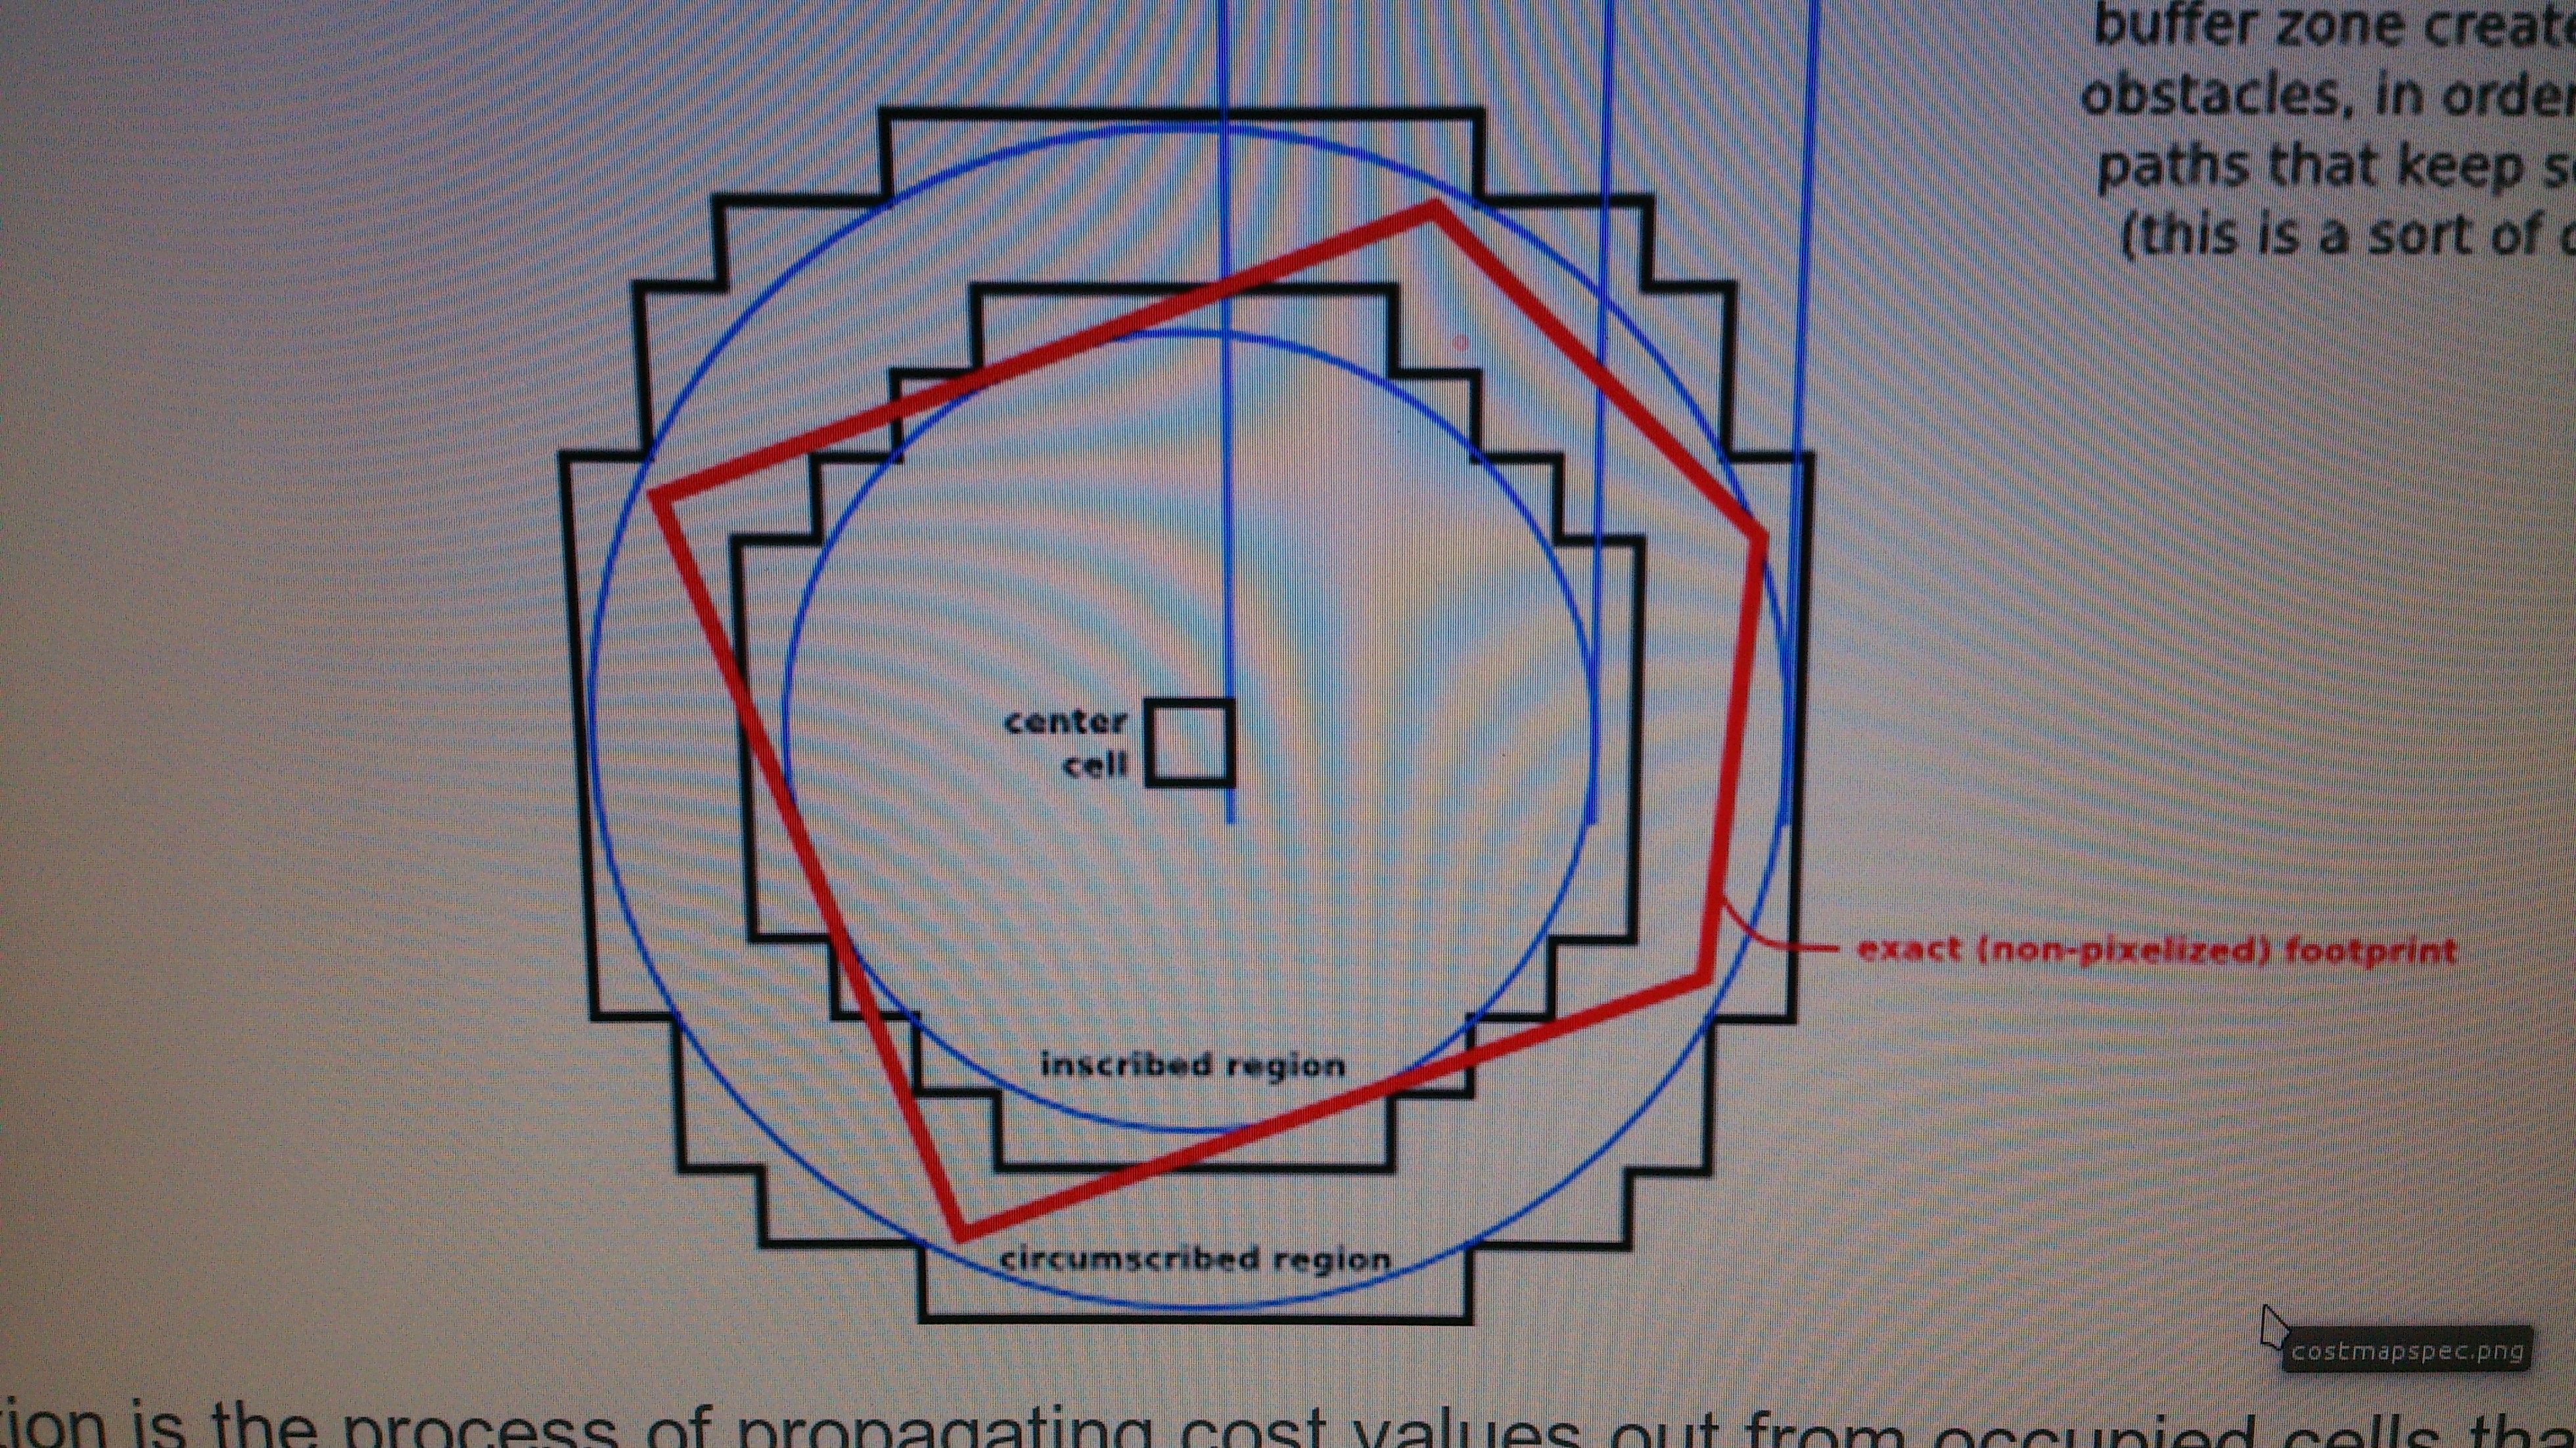
\includegraphics[height=0.5\textheight]{inscribed_circumscribed}
  \end{center}
  
  \note {

  }
\end{frame}

\begin{frame}{Base frame construction}
  \begin{enumerate}
    \item Find the origin of coordinates.
    \item Base frame's arc length $s$ is obtained for each point.
    \item $q$ represents the perpendicular lateral distance respect to the path.
   \end{enumerate}
   \begin{center}
    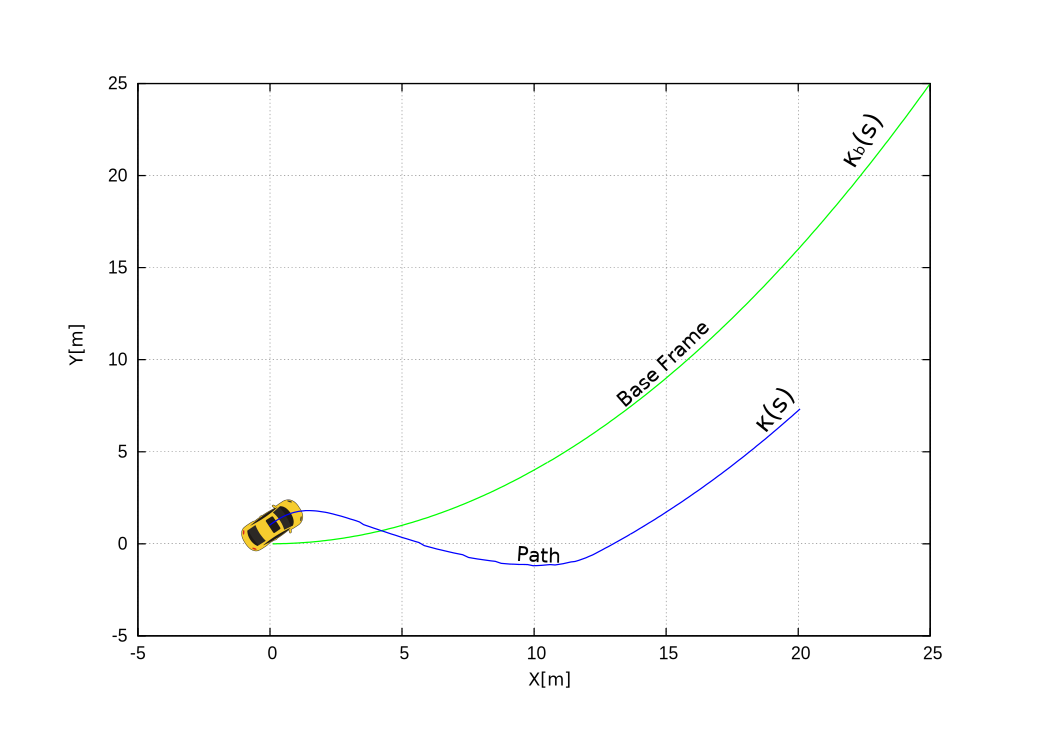
\includegraphics[height=0.5\textheight]{justOneCartesian45}
    ~
    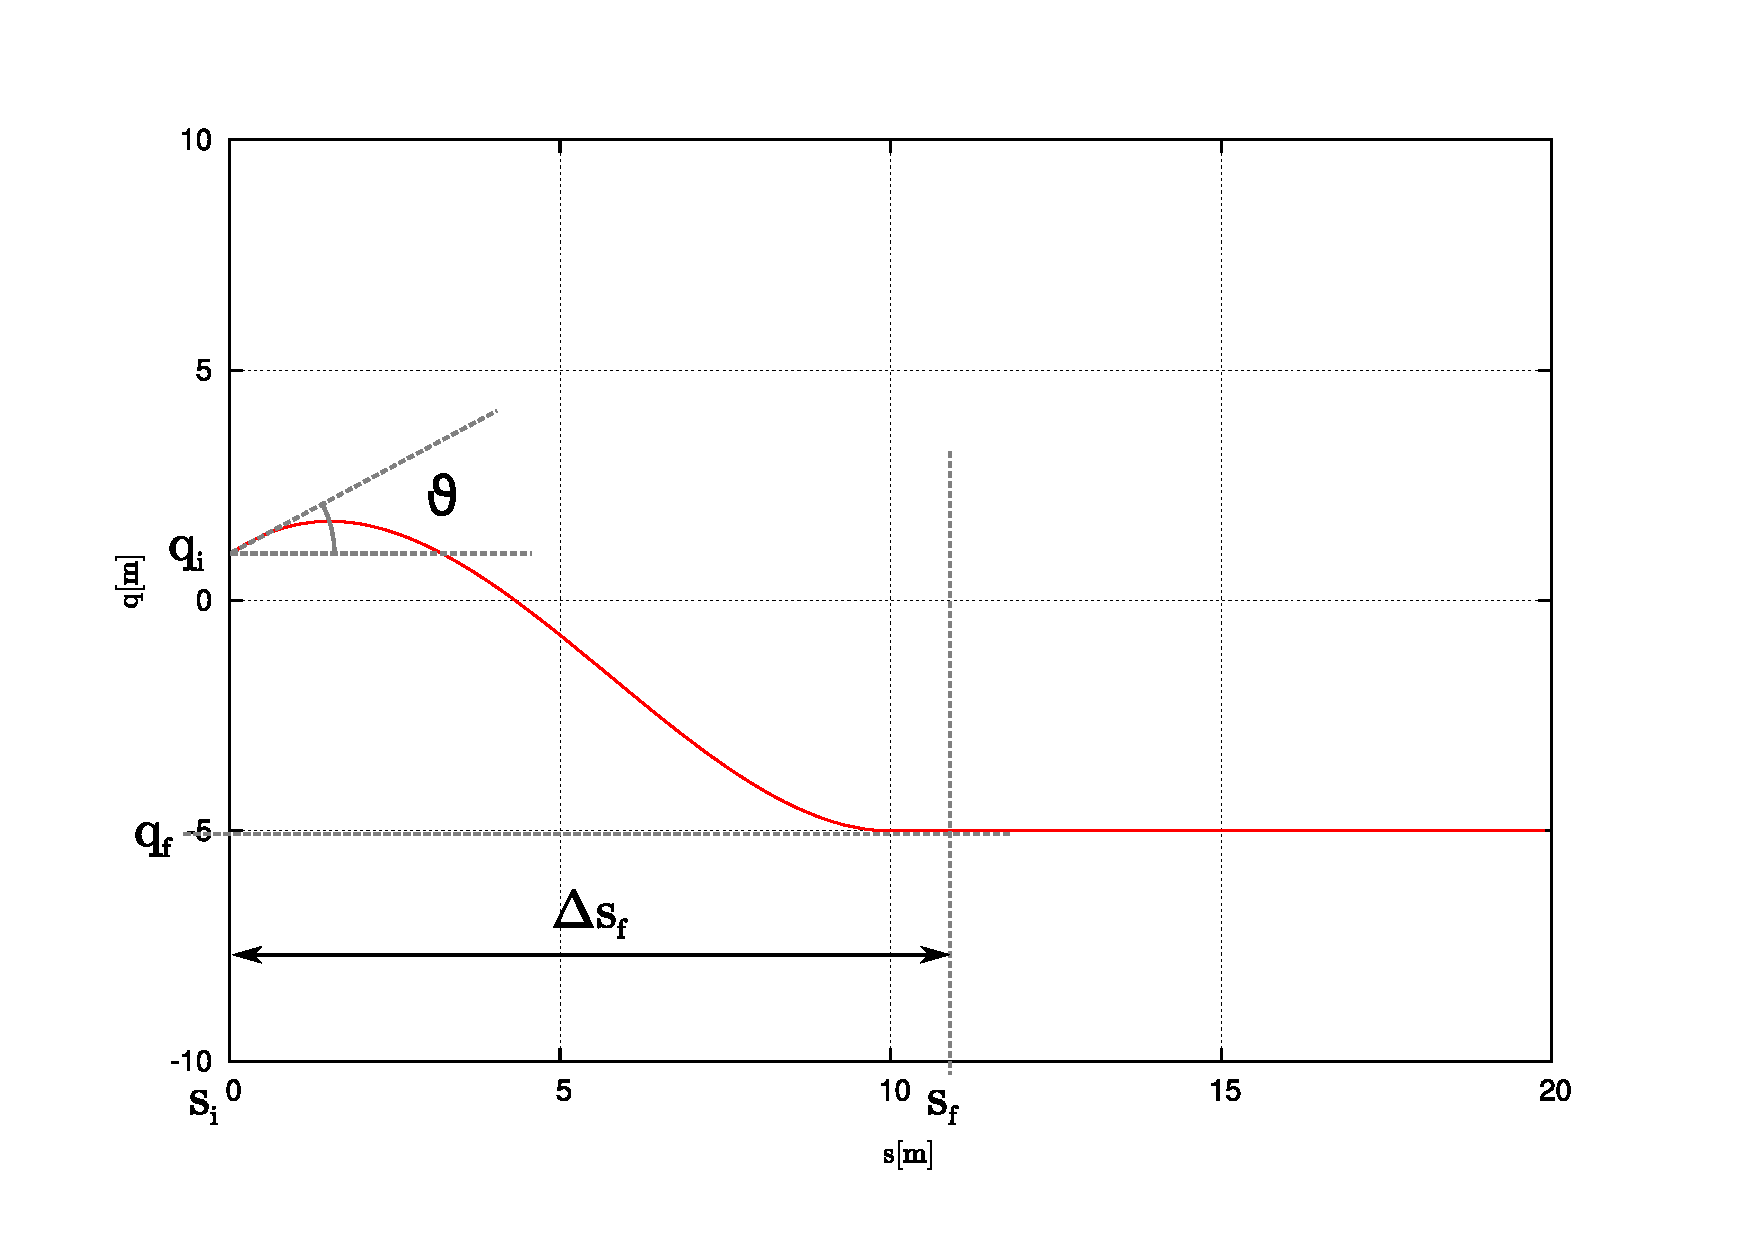
\includegraphics[height=0.5\textheight]{justOneFrenet45}
  \end{center}
  
  \note {

  }
\end{frame}

\begin{frame}{Base frame construction}
  \framesubtitle{Transformation computation}
  \begin{enumerate}
   \item Path curvature $\kappa$ is computed.
   \begin{minipage}[c]{\textwidth}
    \tiny
    \begin{equation}\nonumber
      \kappa = {S \over Q} \cdot \left ( \kappa_b \cdot { 
      {(1 - q \cdot \kappa_b) \cdot (\partial^2q / \partial s^2) +
      \kappa_b \cdot (\partial q / \partial s )^2
      } 
      \over {Q^2} } \right )
      \end{equation}
   \end{minipage}
    \item A path is rejected if $q > {1 \over \kappa_b}$.
    \item Used vehicle motion ignores related physical effects.
      \begin{minipage}[c]{\textwidth}
	  \tiny
	\begin{equation}\nonumber
	  \begin{cases}
	  \dot{x} = |\vec{v}| \cdot cos(\theta) \\
	  \dot{y} = |\vec{v}| \cdot sin(\theta) \\
	  \dot{\theta} = |\vec{v}| \cdot \kappa
	  \end{cases}
	\end{equation}
    \end{minipage}
    \item Speed of the vehicle $\vec{v}$ is removed from the model.
      \begin{minipage}[c]{\textwidth}
	  \tiny
	\begin{equation}\nonumber
	  |\vec{v}| = S \cdot Q \cdot { {\partial s} \over {\partial t}}
	\end{equation}
      \end{minipage}
    \item Differential motion equation becomes:
      \begin{minipage}[c]{\textwidth}
	  \tiny
	\begin{equation}\nonumber
	  \begin{cases}
	    {{\partial x} \over {\partial s}} = Q \cdot cos(\theta) \\
	    {{\partial y} \over {\partial s}} = Q \cdot sin(\theta) \\
	    {{\partial \theta} \over {\partial s}} = Q \cdot \kappa
	  \end{cases}
	\end{equation}
      \end{minipage}
  \end{enumerate}

  
  \note {
    \begin{itemize}
     \item A path is rejected if \item $q > {1 \over \kappa_b}$. In this case, the generated path curvature and sense is opposed to that of the base frame. The path violates the non-holonomic condition of the movement of the vehicle, so it is discarded.
     \item Used vehicle motion ignores related physical effects (like inertia or mass), since they do not affect to the geometric shape of the path. Due to that, we can ignore them in the path generation step. Just two deg. of freedom (v and k)
     \item As we are just interested into the geometric generation of the path, it is possible to remove the speed of the vehicle $\vec{v}$ from the model. This is done by expressing the movement of the vehicle in terms of the traveled distance.
    \end{itemize}

  }
\end{frame}

\begin{frame}{Candidate paths generation}
  \framesubtitle{Maneuvering paths generation}
  \begin{overlayarea}{\textwidth}{\textheight}
    \only<1-> {
    \tiny
    \begin{equation}\nonumber
      \kappa = {S \over Q} \cdot \left ( \kappa_b \cdot { 
      {(1 - q \cdot \kappa_b) \cdot (\partial^2q / \partial s^2) +
      \kappa_b \cdot (\partial q / \partial s )^2
      } 
      \over {Q^2} } \right )
      \end{equation}
    }
    \only<2-> {
      \vskip 0.5cm
      \begin{equation}\nonumber
	\begin{align*}
	q(s) &=
	  \begin{cases}
	  a \cdot \Delta s^3 + b \cdot \Delta s^2 + c \cdot \Delta s + q_i & \text{if } s_i \le s < s_f \\
	  q_f        & \text{if } s_f \le s
	  \end{cases}\\
	{{\partial q} \over {\partial s}}(s) &=
	  \begin{cases}
	  3 \cdot a \cdot \Delta s^2 + 2 \cdot b \cdot \Delta s + c & ~~~~~~~\text{if } s_i \le s < s_f \\
	  0        & ~~~~~~~\text{if } s_f \le s
	  \end{cases}\\
	{{\partial^2 q} \over {\partial s^2}}(s) &=
	  \begin{cases}
	  6 \cdot a \cdot \Delta s + 2 \cdot b & ~~~~~~~~~~~~~~~~~~~~~~~\text{if } s_i \le s < s_f \\
	  0        & ~~~~~~~~~~~~~~~~~~~~~~~\text{if } s_f \le s
	  \end{cases}
	\end{align*}
      \end{equation}
    }
    \only<3-> {
      \begin{center}
	\vskip -0.5cm
	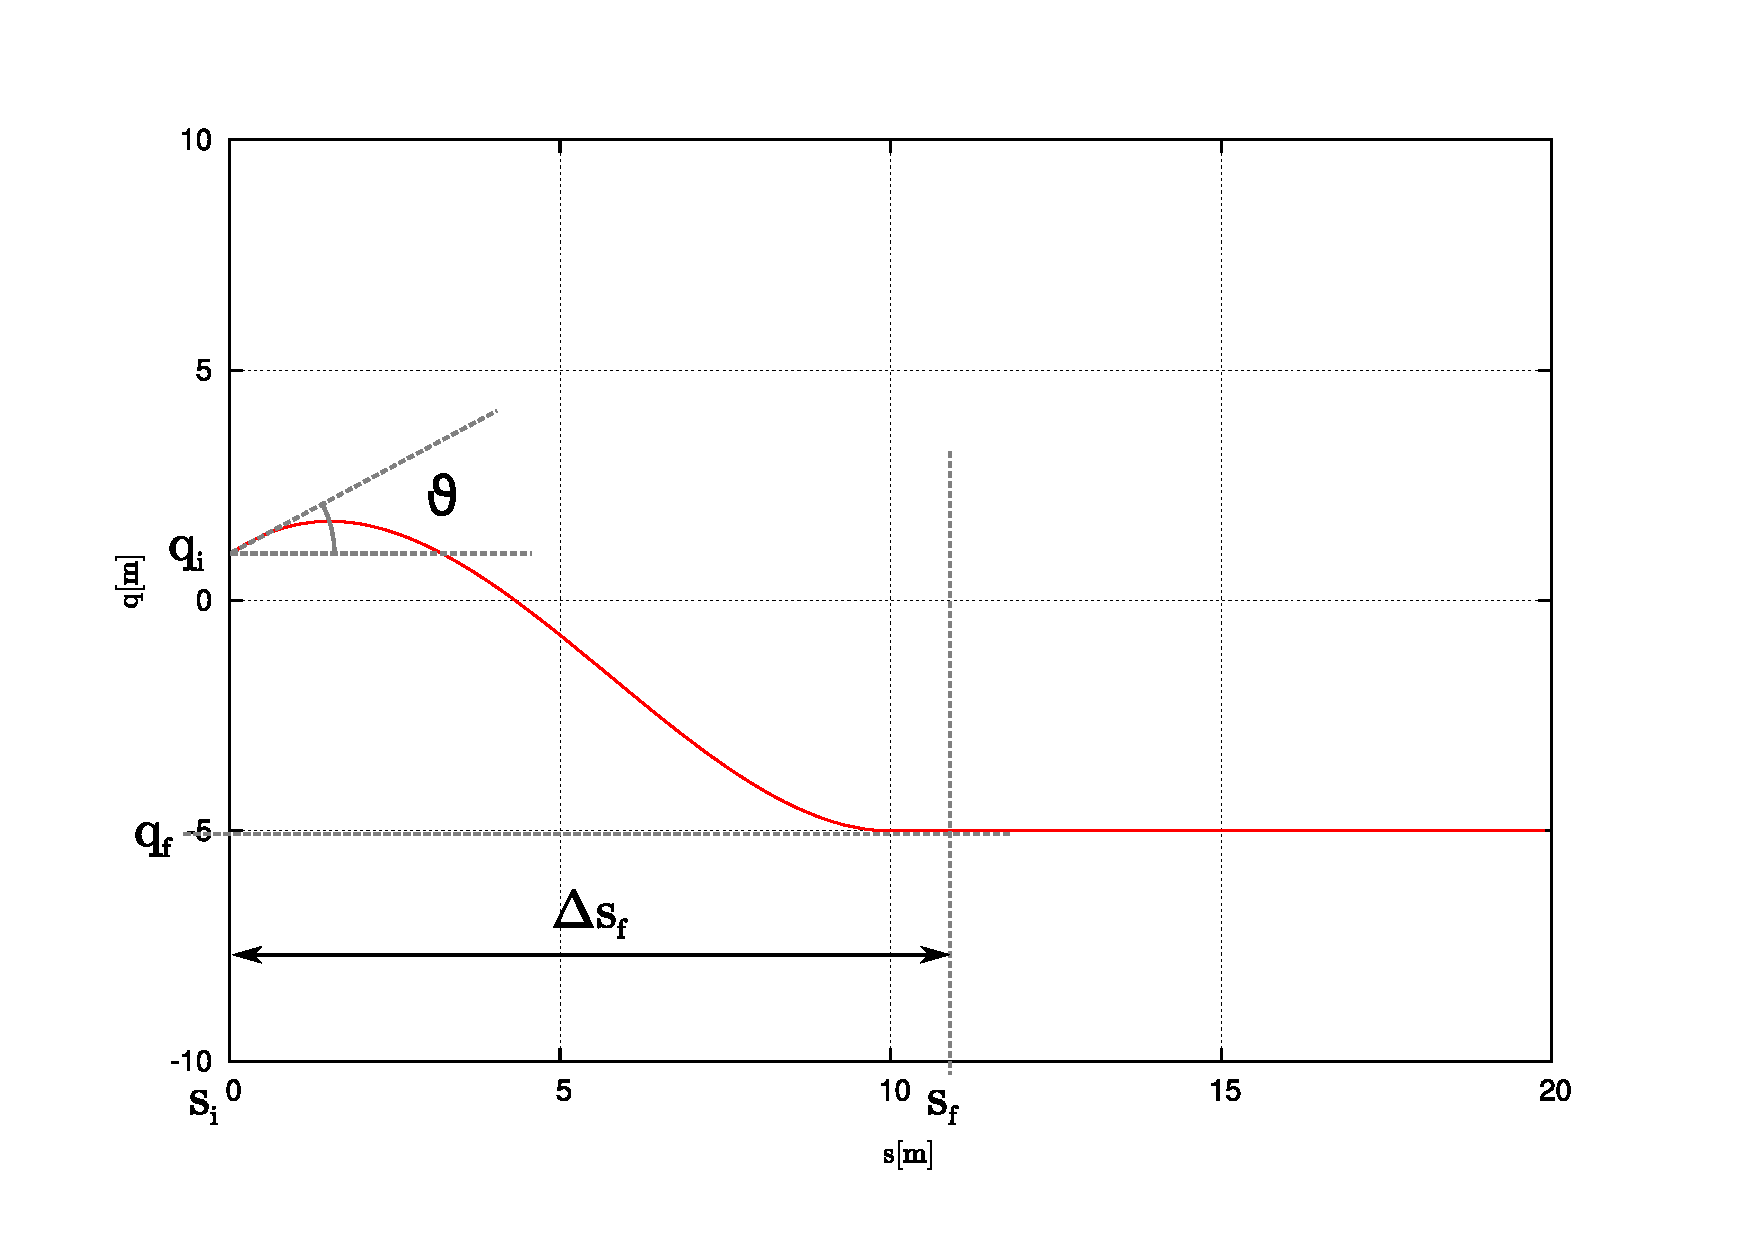
\includegraphics[height=0.4\textheight]{justOneFrenet45}
      \end{center}
    }
    \end{overlayarea}
    

  \note {
    \begin{itemize}
      \item The initial lenght $s_i$ is zero, due to the process performed at the beginning of each iteration (section \ref{ch:chapter07_01_02}). Lateral offset $q_i$ is also known, which is the lateral offset respect to the global path's origin.
      \item Angle $\theta$ defines the difference between the vehicle heading angle and the tangent angle of the base frame at the current position.
      \item $s_f$ is a parameter that allows controlling the longitudinal distance needed to reach the offset $q_f$. This distance should be dependent from the speed. However, as the maximal speed of the prototype is not too hight, we can think on $\Delta s_f$ as the distance needed to go from $q_i$ to the biggest $q_f$ at the maximal speed.
      \item The different $q_f$ are computed separately for each path attending to the parameters defined by the user. $s_f$ is also a free parameter.      
    \end{itemize}
    
    Parameters $s_i$, $q_i$, and $s_f$ are shared by all candidate paths. By modifying the value of $q_f$ we get different tentative trajectories, so the only difference between all them is the lateral offset we want to reach at the end of paths. This lateral offset will give us flexibility in the way in which we avoid obstacles. To do that, we divide the width of the road into as many segments as paths are desired. $q_f$ will be the perpendicular distance between the base frame and the corresponding road width division. Using this technique, the desired number of paths is created. The set of paths should cover the whole road width, ensuring the vehicle is able to avoid the obstacles, if it is possible.

    In our tests, we have considered a maximal width of 4\,m (a little bit above the width of the roads in our testing area), and an horizon of 10\,m in the direction of the global path. This horizon gives us a prediction of 2\,seconds at the maximal speed of the vehicle. We evaluate a total of 21 paths, with a distance between them ($\Delta q_f$) of 20\,cm.

  }
\end{frame}

\begin{frame}{Candidate paths generation}
  \framesubtitle{Candidate paths generation}
    
  \begin{itemize}
   \item Paths are transformed from Frenét space to Euclidean.
  \end{itemize}

  \begin{figure}
    \centering
    \begin{tabular}{cc}
      \begin{subfigure}[b]{0.3\textwidth}
	\centering
	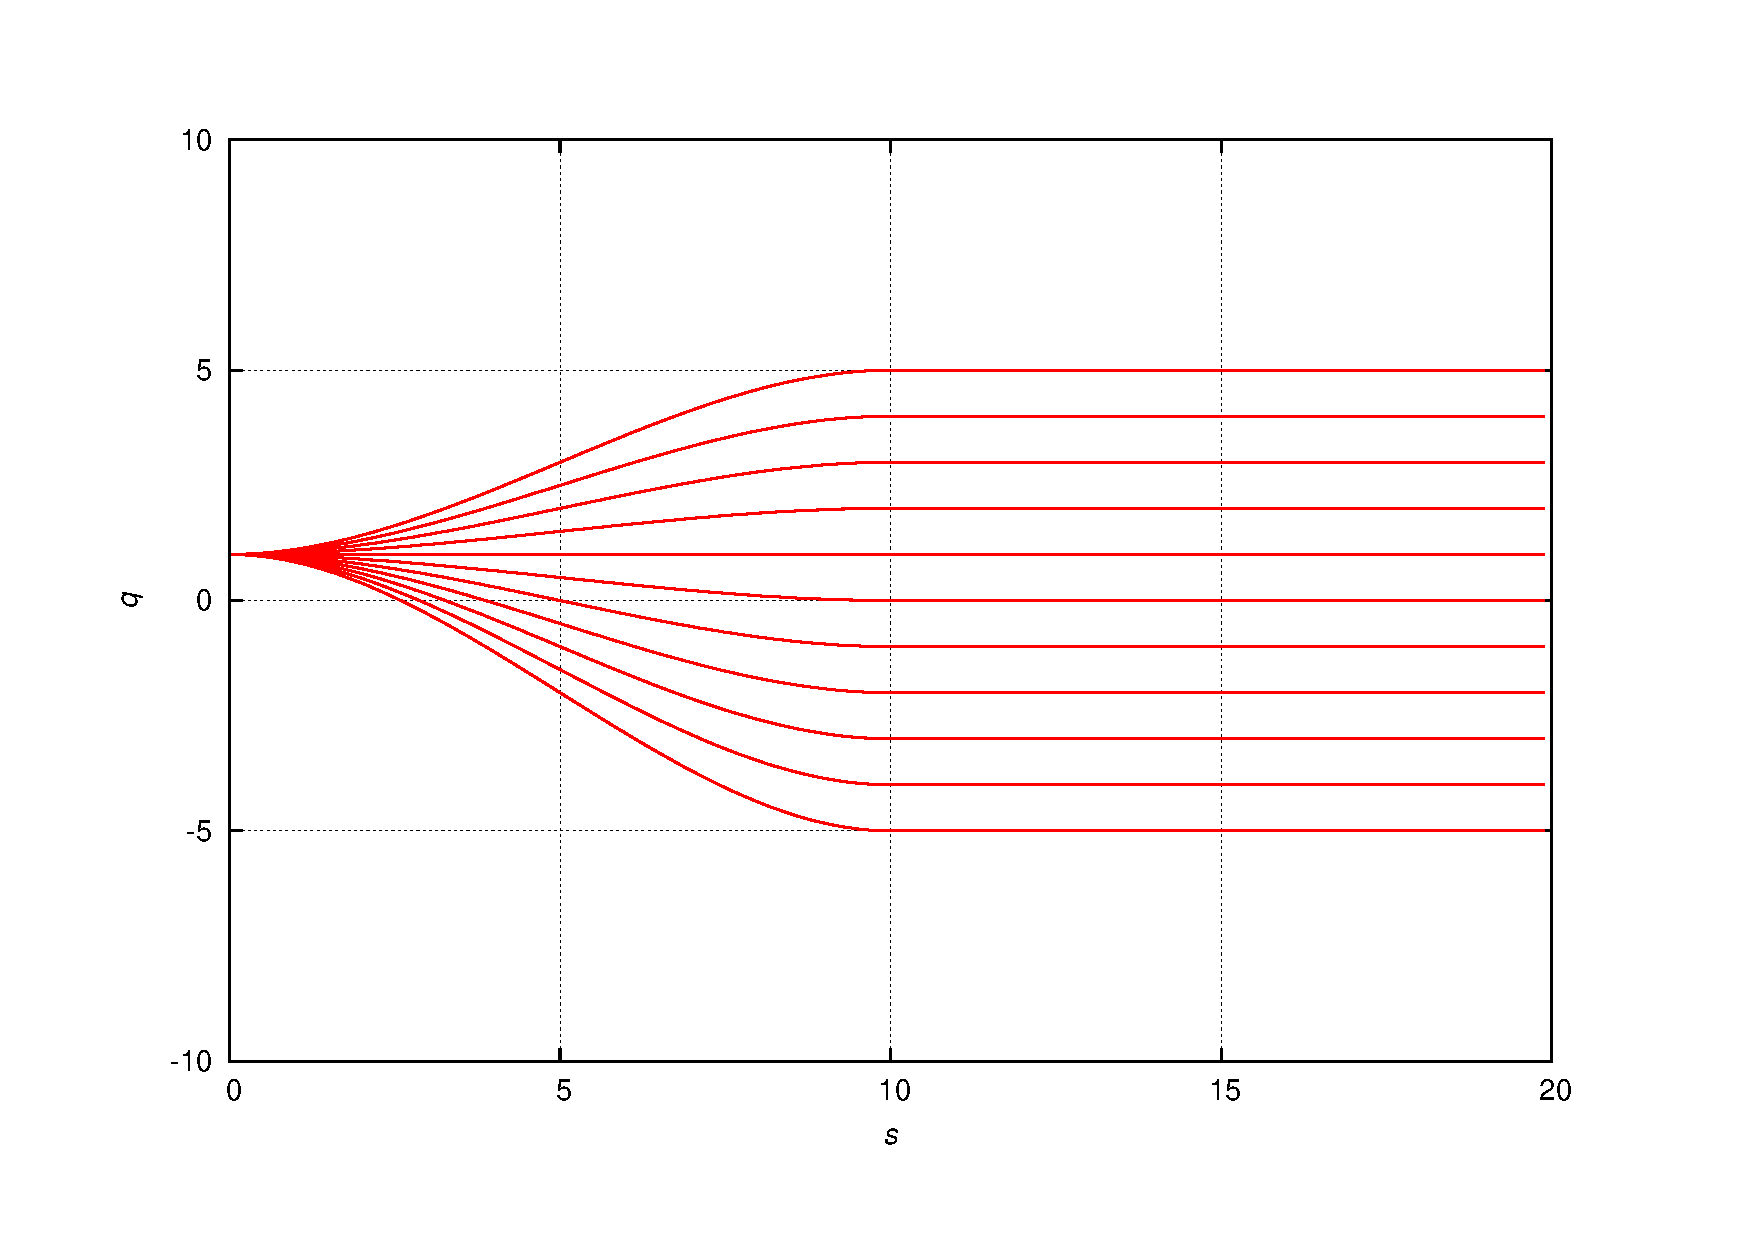
\includegraphics[height=0.3\textheight, trim=50 40 80 60,clip]{frenet0}
      \end{subfigure} &
      \begin{subfigure}[b]{0.3\textwidth}
	\centering
	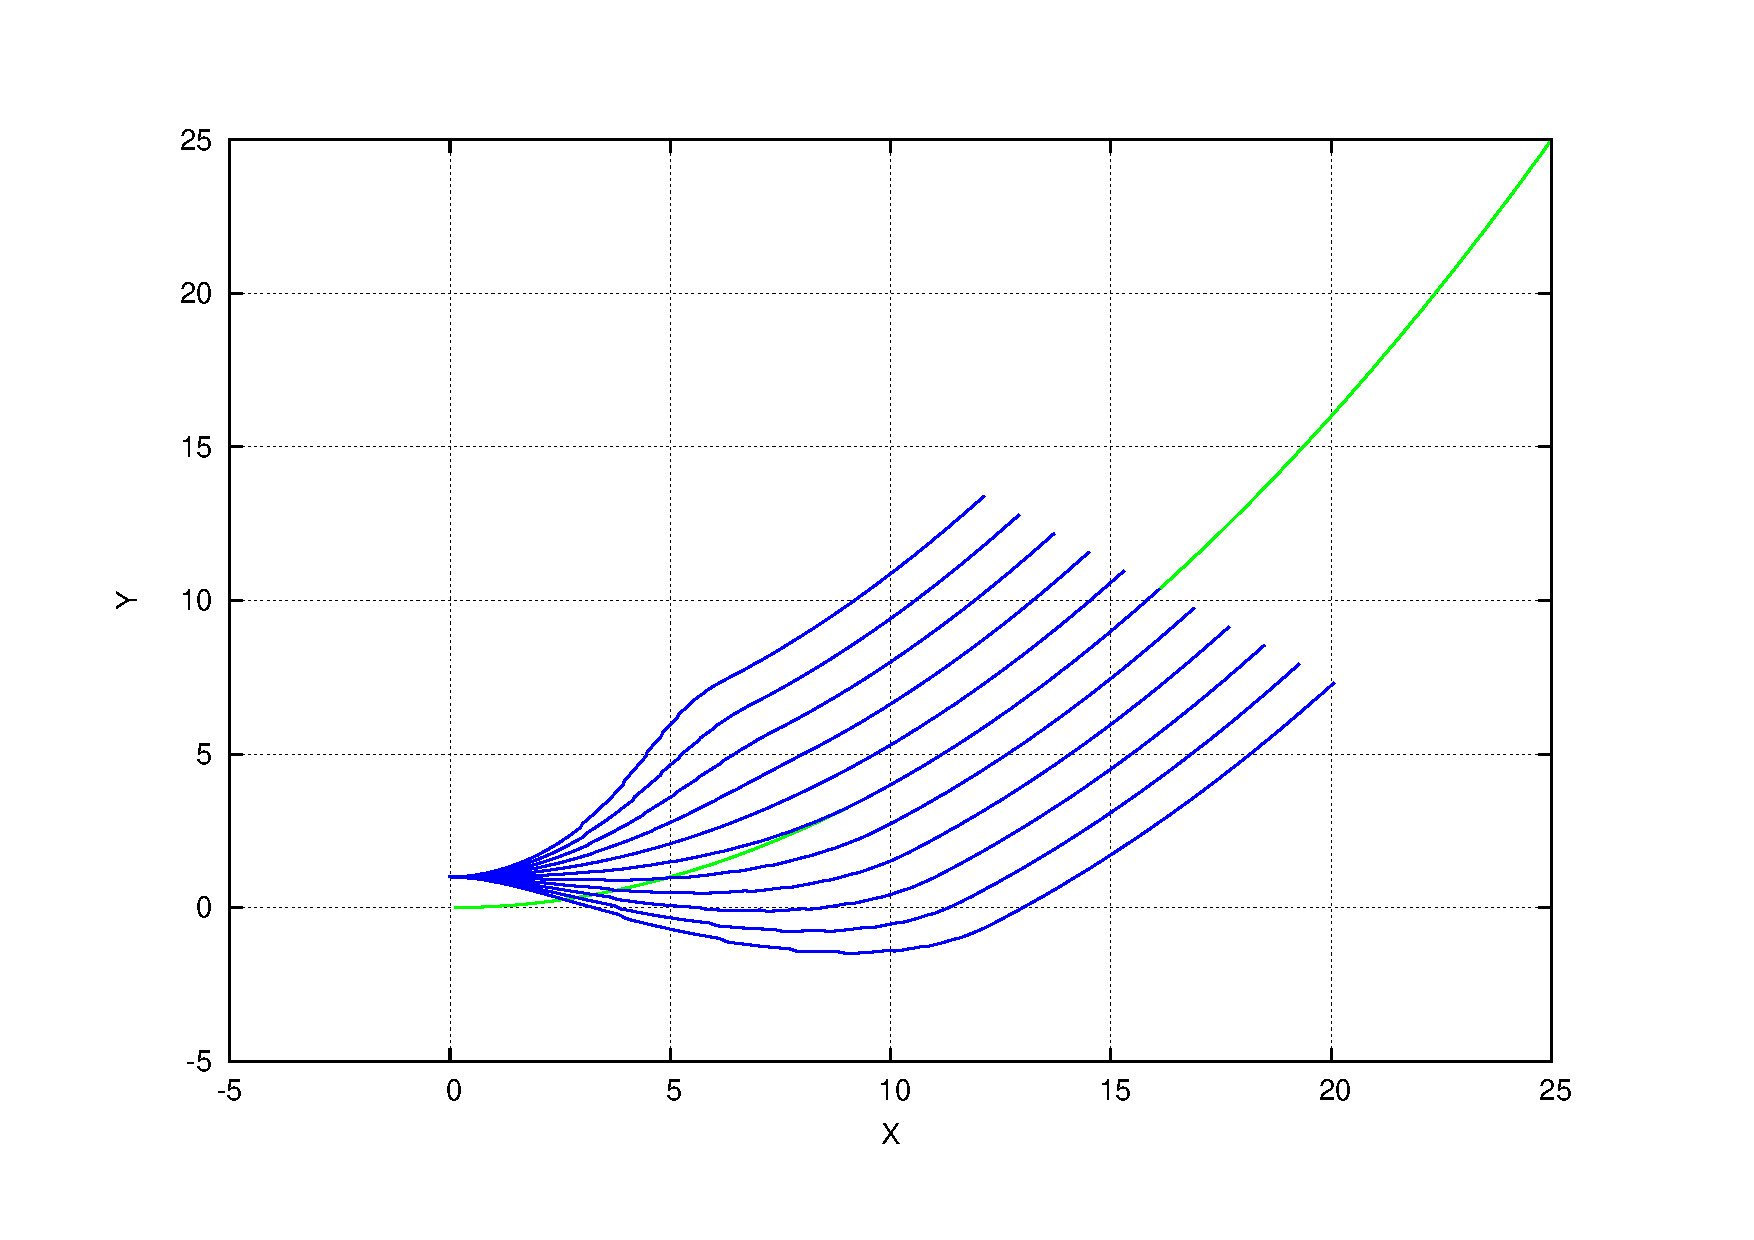
\includegraphics[height=0.3\textheight, trim=50 40 80 60,clip]{cartesian0}
      \end{subfigure}%
    \end{tabular}
  \end{figure}

  \begin{figure}
  \centering
  \begin{tabular}{cc}
    \begin{subfigure}[b]{0.3\textwidth}
      \centering
      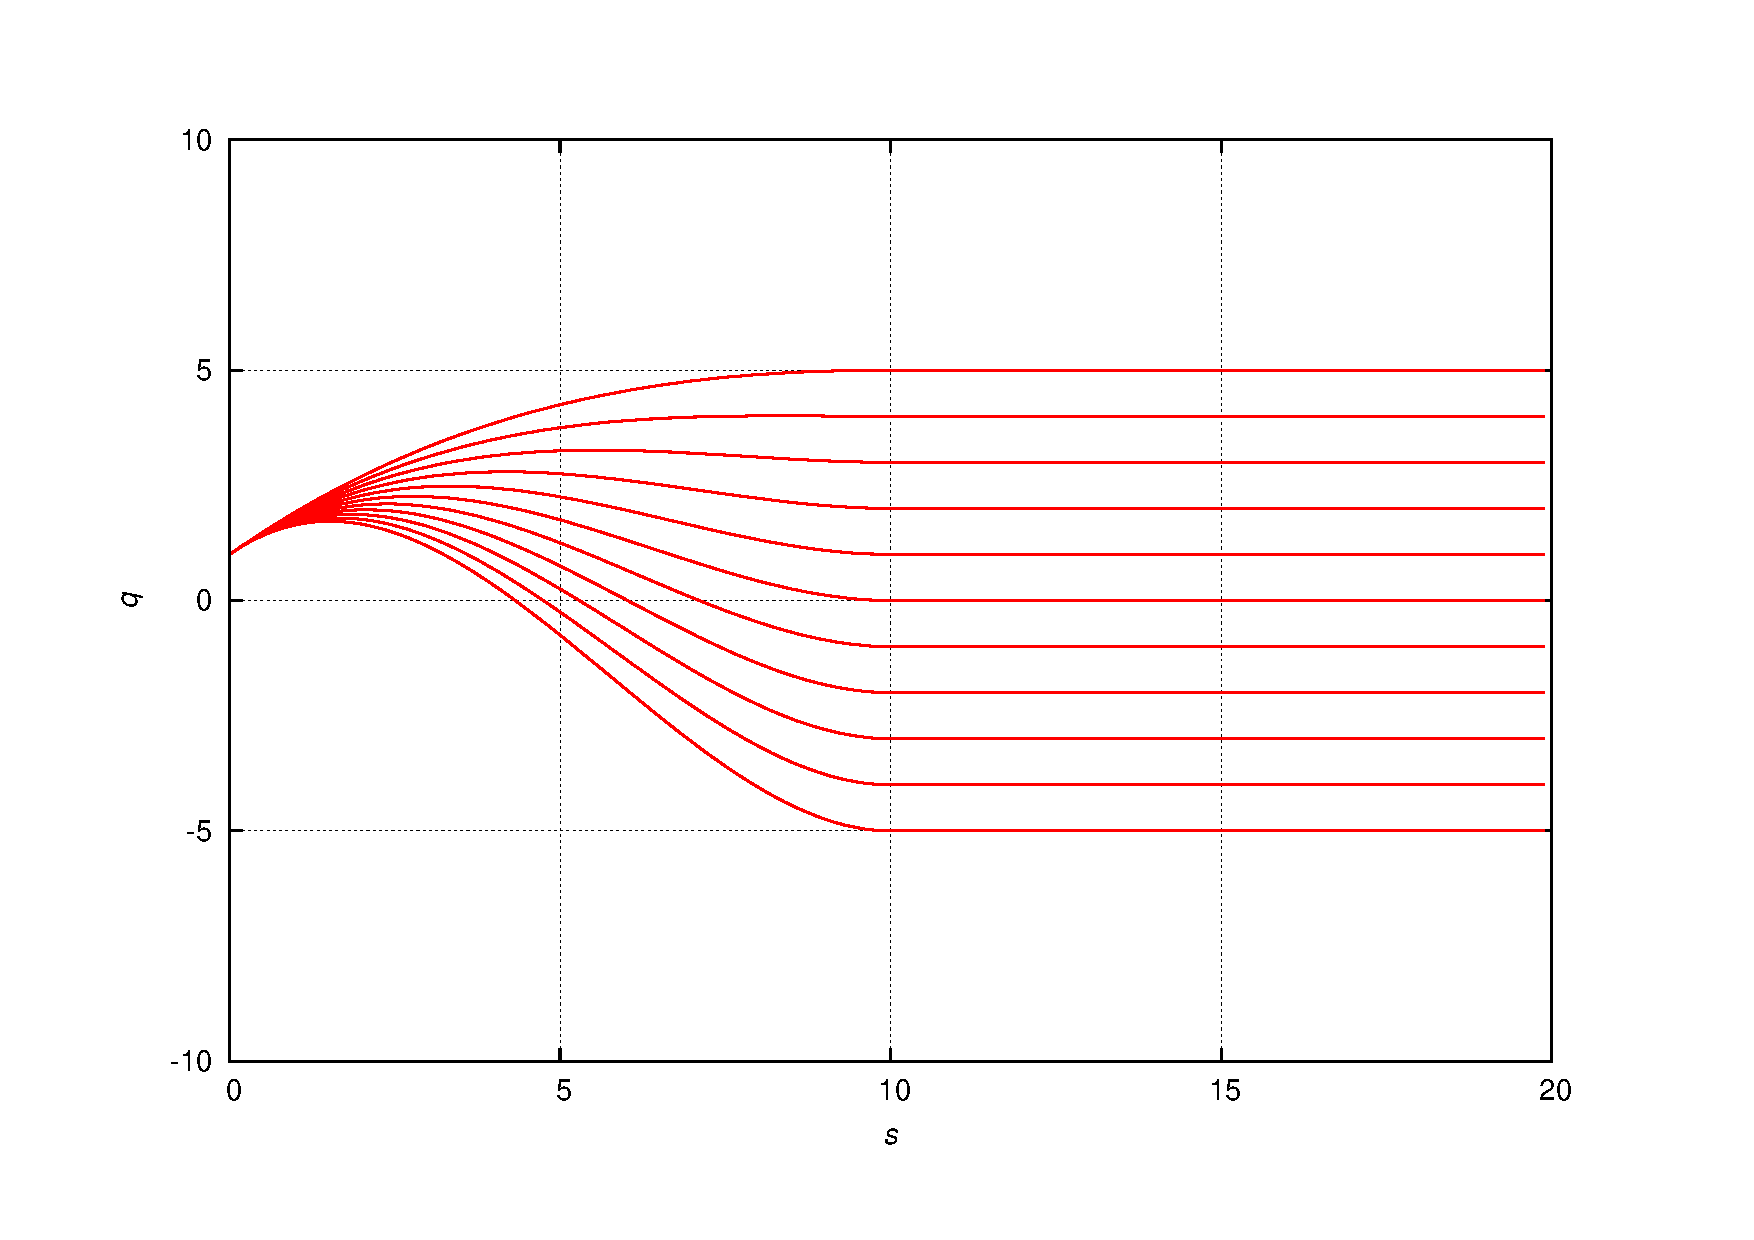
\includegraphics[height=0.3\textheight, trim=50 40 80 60,clip]{frenet45}
      \caption{Curvilinear space.}
    \end{subfigure} &
    \begin{subfigure}[b]{0.3\textwidth}
      \centering
      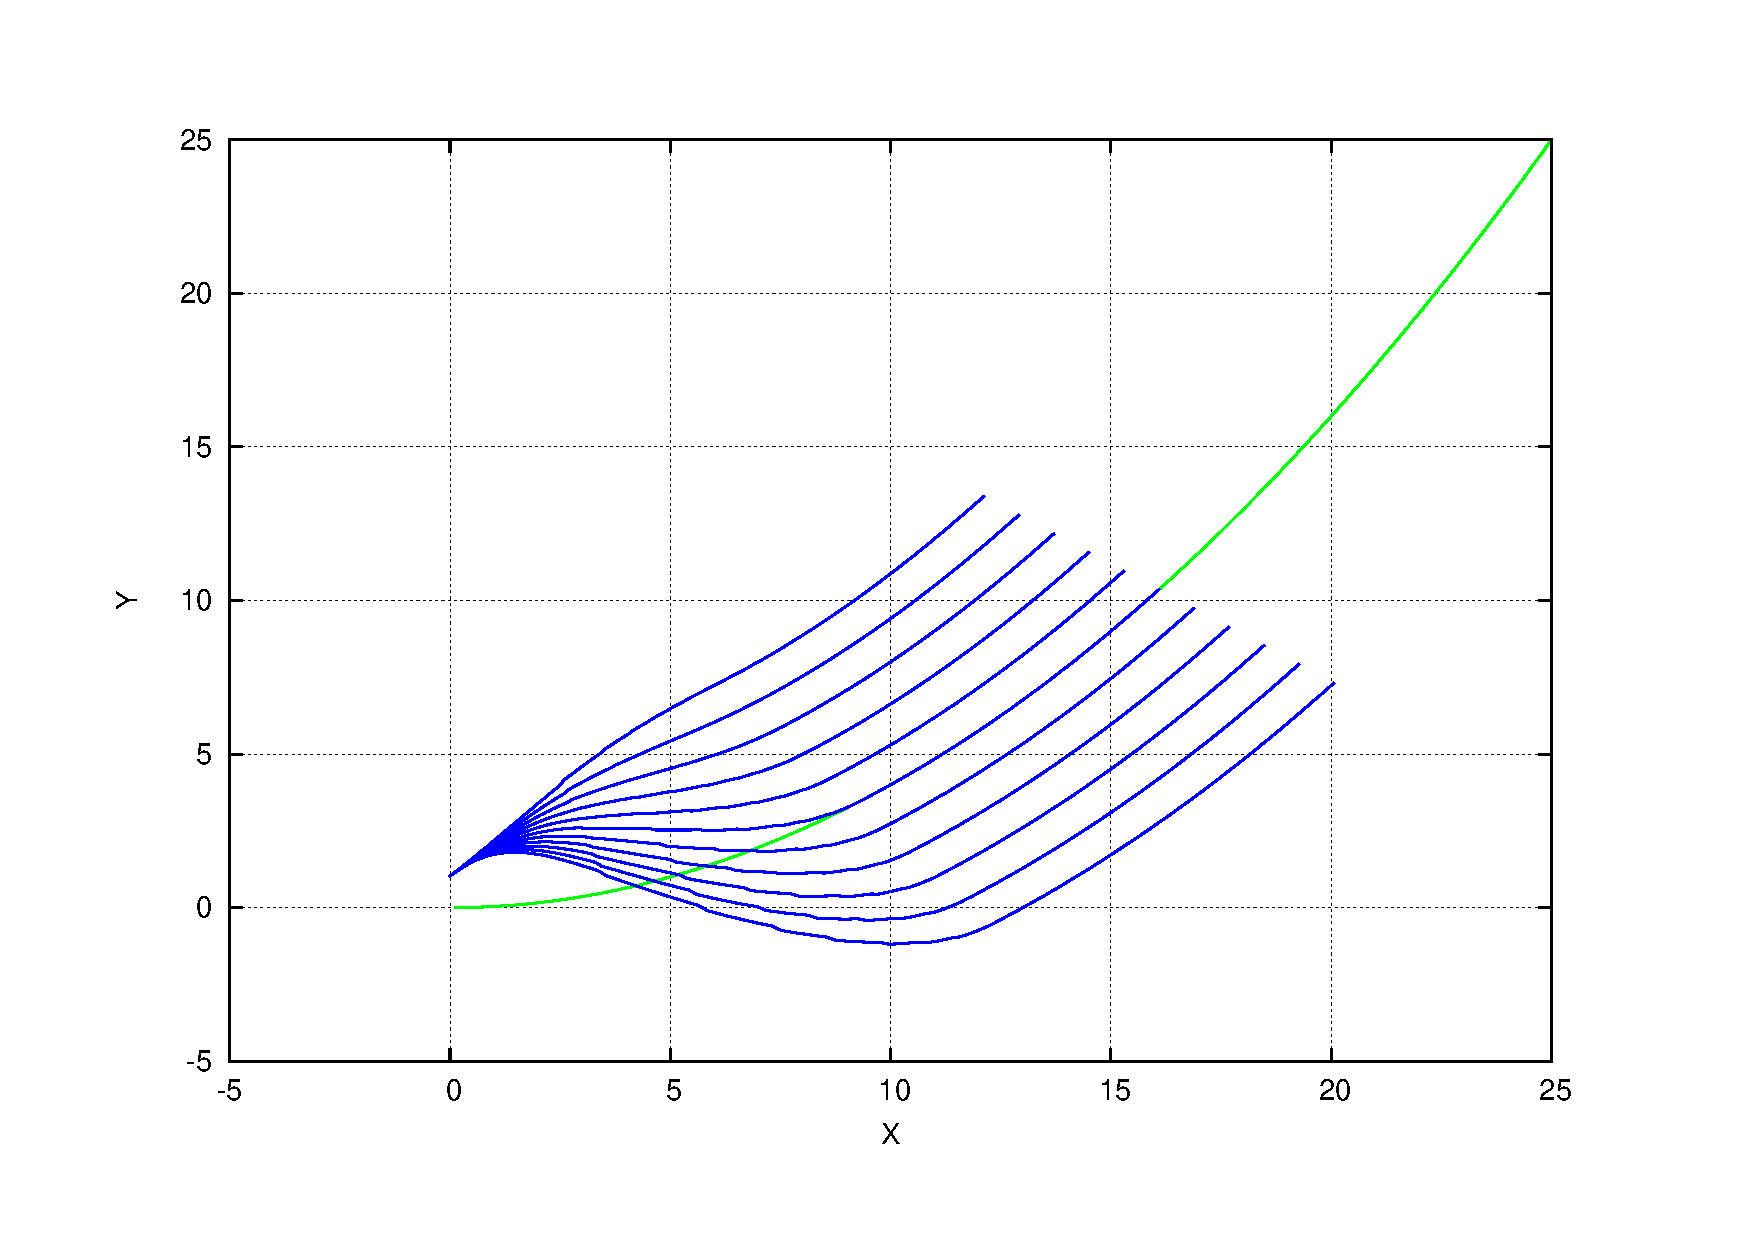
\includegraphics[height=0.3\textheight, trim=50 40 80 60,clip]{cartesian45}
      \caption{Euclidean space.}
      \end{subfigure}
  \end{tabular}
  \end{figure}
  \note {
    
  }
\end{frame}

\begin{frame}{Candidate paths generation}
  \framesubtitle{Winner path selection}
    
  \begin{itemize}
    \only<1> {
    \item Linear combination $J[i]$ of weighted cost functions:
    \begin{minipage}[c]{\textwidth}
      \vskip 0.5cm
      \begin{equation}\nonumber
	J[i] = \omega_o C_o[i] + \omega_l C_l[i] + \omega_d C_d[i] + \omega_{\kappa} C_{\kappa}[i] + \omega_c C_c[i]
      \end{equation}
    \end{minipage}
    \vskip 1.0cm
    \item All costs $C_o$, $C_l$, $C_d$, $C_{\kappa}, C_c$ normalized to 1.0, and
    \begin{minipage}[c]{\textwidth}
      \vskip 0.5cm
      \begin{equation}\nonumber
	\sum_{{i \in \{o, l, d, \kappa, c\}}} w_i= 1.0
      \end{equation}
      \vskip 0.5cm
    \end{minipage}
    }
    \only<2> {
    \item Costs:
    \begin{itemize}
     \item Occlussion: $C_o = {{max\{c_i\}} \over 255}, ~~~~~~ i=1 \dots L$
     \item Length: $C_l = 1- {{\sum\limits_{i=1}^{L}\|p_i - p_{i - 1}\|} \over {q_{f_{max}} + s_f}}$
     \item Distance to global path: $C_d = {{\sum\limits_{i=1}^{L}\|p_i - nearest(p_i, g)\|} \over {L \cdot q_{f_{max}}}}$
     \item Curvature: $C_{\kappa} = max \left \{ {{x_i' \cdot y_i'' - x_i'' \cdot y_i'} \over {(x_i' + y_i')^{3/2}}} \right \}, ~~~~~~ i=1 \dots L$
     \item Consistency: $C_c = {1 \over {s_2 - s_1}} \int \limits_{s_1}^{s_2} l_i ~ ds$
    \end{itemize}
  }
  \end{itemize}

  
  \note {
    
  }
\end{frame}

\begin{frame}{Computation of vehicle commands}
  \begin{itemize}
    \item A PID controller is tuned.
    \item We want to minimize the distance and heading of the vehicle respect to the trajectory.
    \item Computed values are sent to vehicle.
  \end{itemize}

\end{frame}

\begin{frame}[plain]{Local planning}
  \begin{columns}[c] % the "c" option specifies center vertical alignment
  \column{.5\textwidth} % column designated by a command
  \includemovie[autoplay, repeat]{\linewidth}{.75\linewidth}{/home/nestor/Seafile/Videos/Tesis/cp02/trackingParking.mp4}
  \includemovie[autoplay, repeat]{\linewidth}{.75\linewidth}{/home/nestor/Seafile/Videos/Tesis/cp02/trackingParking.mp4}
  \column{.5\textwidth}
  \includemovie[autoplay, repeat]{\linewidth}{.75\linewidth}{/home/nestor/Seafile/Videos/Tesis/cp02/EPFL.mp4}
  \includemovie[autoplay, repeat]{\linewidth}{.75\linewidth}{/home/nestor/Seafile/Videos/Tesis/cp02/trackingParking.mp4}
  \end{columns}
\end{frame}
